\section{Approach Overview}
\label{section:overview}

To address the challenges of pipeline stage imbalance and training data dynamicity,
we introduce \underline{D}ynamic \underline{I}nterleaved \underline{P}ipeline (\sys{}), a dynamic and modality-aware scheduling framework designed to optimize pipeline parallelism for LMMs.
\sys{} is built on three key design principles:
asynchronous schedule generation to hide search latency,
modality-aware partitioning to mitigate imbalance at its source, and
decomposed search algorithm to find high-quality pipeline schedules efficiently.

\subsection{Design Principles}
\label{section:design-decisions}

\begin{figure}[b]
    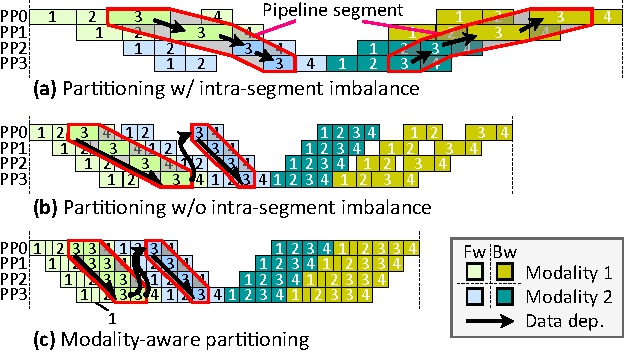
\includegraphics[width=1.0\columnwidth]{./figures/svg/schedule_observations.pdf}
    \caption{
        Illustrations of partitioning schemes from \S\ref{section:design-decisions}.
        Numbers in boxes denote microbatches.
        \textbf{(a)} Non-modality-aware partitioning co-locates stages from different modalities in the same pipeline segment, causing intra-segment imbalance.
        \textbf{(b)} Separated partitioning dedicates distinct pipeline segments to each modality, removing intra-segment imbalance.
        \textbf{(c)} Modality-aware data batching further splits microbatches into smaller, modality-specific sub-microbatches to balance workloads across segments.
    }
    \label{figure:schedule-observations}
\end{figure}

\heading{Asynchronous Schedule Generation}
In contrast to conventional approach\-es that rely on static or pre-computed schedules, \sys{} adopts an online, asynchronous strategy,
in order to handle the dynamic nature of LMM data.
For each upcoming data batch, it concurrently generates a tailored pipeline schedule on-the-fly, effectively adapting to the fluctuating computational demands of multimodal data.
This process, which includes data prefetching and schedule searching, runs asynchronously on idle CPU resources, parallel to the main training workers on GPUs. By staying off the critical path, our approach provides the adaptability needed for dynamic data without introducing significant overhead.

\heading{Modality-Aware Partitioning}
The primary source of inefficiency in LMM training stems from the dynamic computational imbalance between different modality modules, as discussed in \S\ref{section:dynamic-imbalance}.
Such dynamic imbalance creates irregular stage latencies and makes it difficult to remove pipeline bubbles.
% Merely optimizing the scheduling order is insufficient, since significant disparities in stage latencies across modality modules make it difficult to eliminate pipeline bubbles.
To address this, \sys{} aims to reduce pipeline bubbles at their source by minimizing stage latency discrepancies.
This is achieved through partitioning the computation of different modality modules into equally-wide \emph{pipeline segments}.
Our approach is guided by two key techniques:

\textbf{\ding{172} Remove Intra-Segment Imbalance with Separated Partitioning.}
A \emph{pipeline segment} is a set of consecutive stages distributed across all $P$ pipeline ranks.
For example, the four forward stages numbered with ``3'' in \figref{figure:schedule-observations}a form one pipeline segment,
while their corresponding backward stages form another one.
We observe that co-locating stages from different modality modules within the same segment (\figref{figure:schedule-observations}a) is inherently inefficient. Because vision and language stages have different computational costs and sensitivities to data proportions (\eg number of images vs. tokens), mixing them creates unavoidable latency disparities between pipeline ranks. Our first principle is to enforce \emph{separated partitioning} (\figref{figure:schedule-observations}b), where each modality module occupies its own dedicated pipeline segments. This eliminates a primary source of pipeline bubbles. For the ViT 2B + LM 5B model (\S\ref{section:dynamic-imbalance}), this strategy alone improves performance by 13.1\% over the best mixed partitioning scheme.

\textbf{\ding{173} Remove Inter-Segment Imbalance with Modality-Aware Batching.}
After separating modalities, we must balance the workload between their respective segments. Our second principle is to partition data within a microbatch into smaller, modality-specific \emph{sub-microbatches} (\figref{figure:schedule-observations}c). For example, if the entire vision encoder stage is slower than a LM stage, we can process images in smaller sub-microbatches.
This allows the encoder to execute multiple shorter stages, and each encoder stage latency can be tailored to better match the latency of a single LM stage.
This modality-aware batching reduces latency discrepancies across the entire pipeline, enabling a more globally balanced and efficient schedule.

\heading{Decomposed and Scalable Schedule Search}
The scheduling search problem can be formulated as a monolithic integer linear program (ILP) and solved with off-the-shelf solvers~\cite{highs,gurobi}.
This approach is precise but intractable for real-time use, often taking minutes or hours to solve~\cite{recycle-sosp24}.
To meet the tight time budget of a single training iteration (typically 10--60 seconds, \figref{figure:e2e-perf}b), we adopt a divide-and-conquer strategy that decomposes the complex search problem into a sequence of simpler, more manageable subproblems. As shown in \figref{figure:plan-searcher}, our searcher iterates through a three-phase loop, applying tailored heuristics at each step:

\textbf{\ding{172} Pipeline Segment Reordering (\S\ref{section:segment-reordering}):} First, we determine the optimal processing sequence of pipeline segments. We use Monte Carlo Tree Search (MCTS) to efficiently explore the vast permutation space and identify promising pipeline segment orderings.

\textbf{\ding{173} Pipeline Stage Interleaving (\S\ref{section:stage-interleaving}):} With a fixed segment order, we then arrange the corresponding forward and backward pipeline stages. A fast, dual-queue greedy algorithm interleaves these stages to minimize pipeline bubbles and pack the schedule tightly.


\textbf{\ding{174} Per-Layer Memory Optimization (\S\ref{section:memory-optimization}):} Finally, with the schedule structure fixed, we optimize memory usage independently on each pipeline rank. This phase selects memory-saving strategies (e.g., activation checkpointing and offloading) for all model layers to minimize memory usage fluctuations induced by data dynamicity and optimize end-to-end iteration latencies.

This entire loop is highly parallelizable across CPU threads, ensuring that our search process scales with available CPU resources and can serve large distributed training clusters.

\subsection{System Workflow}
\label{section:dip-overview}

The principles above are orchestrated by the \sys{} training planner, which consists of three main components: modality-aware partitioner (\S\ref{section:modality-aware-partitioning}), pipeline schedule searcher (\S\ref{section:pipeline-schedule-searcher}), and training simulator (\S\ref{section:multimodal-training-simulator}).

\begin{figure}[t]
    
\includegraphics[width=0.95\columnwidth]{./figures/svg/overview.pdf}
    \caption{
        The overall workflow of \sys{}.
        Before training, the LMM model is partitioned into model chunks by the model chunk partitioner.
        During each training iteration, \sys{} asynchronously executes a four-stage online planning process.
    }
    \label{figure:overview}
\end{figure}

\begin{figure}[t]
    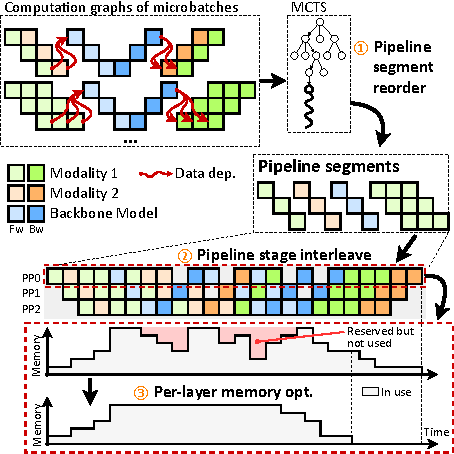
\includegraphics[width=1\columnwidth]{./figures/svg/plan_searcher.pdf}
    \caption{
        The workflow of \sys{}'s pipeline schedule searcher.
    }
    \label{figure:plan-searcher}
\end{figure}

The overall workflow proceeds in two phases, as shown in \figref{figure:overview}.
The modality-aware partitioner comprises an offline model chunk partitioner and an online sub-microbatch partitioner.
\textbf{Before training,} the model chunk partitioner divides the LMM into model chunks based on our separated partitioning principle and distributes them to the designated GPUs.
\textbf{During training,} all model chunks remain statically placed on their respective GPU workers, which also fixes the underlying network topology (\eg NCCL connections).
For each iteration, the planner executes a four-stage process:

\textbf{\ding{172} Metadata Prefetching:} The planner fetches metadata for the next batch (\eg token counts, number of images).

\textbf{\ding{173} Adaptive Microbatch Partitioning:} Using this metadata, the sub-microbatch partitioner divides the microbatches into smaller, modality-specific sub-microbatches to enable inter-segment load balancing.

\textbf{\ding{174} Pipeline Schedule Search:} Pipeline schedule searcher is guided by performance estimates from the simulator and runs its three-phase algorithm to find an optimal schedule for the generated sub-microbatches.

\textbf{\ding{175} Runtime Deployment:} The best schedule is compiled into an execution plan and dispatched to the distributed training runtime for execution.

% This dynamic, interleaved pipeline allows \sys{} to continuously adapt to data variations, maintaining high training efficiency for complex LMM workloads.
